\label{sec:choiceOfMethod}
Figure \ref{fig:methods} shows an overview of various research methods and three criteria that can be used to determine the appropriate research method. The criteria are: form of research question, whether the study requires control of behavioural events and if the study focuses on contemporary events. The defined research question for this study, as presented in section \ref{sec:objectives}, is a so-called "how" question. As the goal of our study is to reveal current practices in organizations, we do not need control over behavioural events. The study focuses mainly on contemporary events. Some past events such as incidents that have occurred are relevant, but the main focus is on current practices. Based on this, case study emerged as the most suitable method for this study, as highlighted in the figure.

A case study is applicable to real-world organizations, which is what we wanted to study. An advantage is that it can deal with various kinds of evidence, such as documents, archival records, interviews and artefacts.

\begin{figure}[h]
\begin{center}
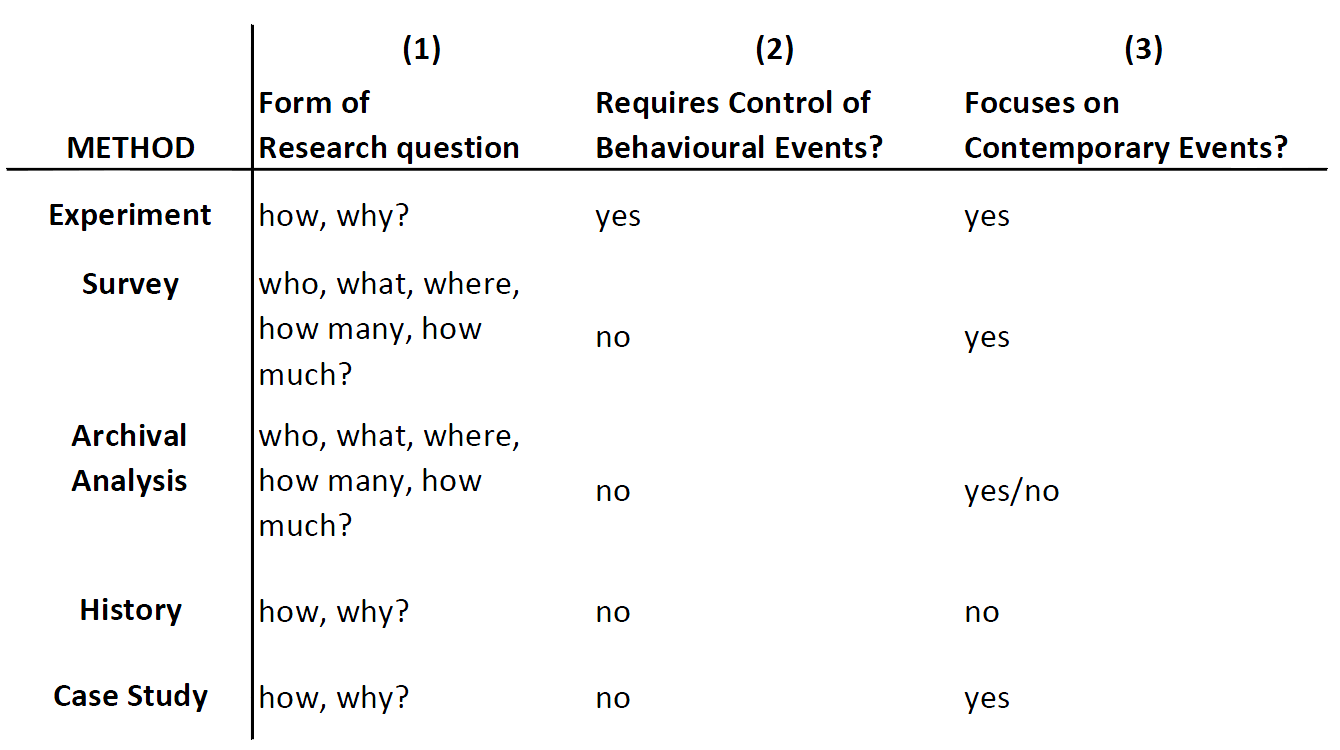
\includegraphics[scale=0.35]{methods.png}
\caption[Choice of Research Method]{Choice of Research Method, modified from \cite{CaseStudyResearch}}
\label{fig:methods}
\end{center}
\end{figure}

